%\documentclass[a4paper,11pt]{article}
\documentclass[a4paper,twocolumn]{article}
%\documentclass[a4paper,11pt,landscape,twocolumn]{article}
%\documentclass[a4paper]{memoir}
\usepackage[utf8]{inputenc}
\usepackage[spanish, es-tabla, es-nodecimaldot]{babel}
\usepackage{amsmath}  %permite usar \text{} en el entorno Matemática
\usepackage{amssymb} % para el de números reales
%\usepackage{fancyhdr} %para encabezados y pies de página lindos
%\usepackage{lastpage} %para poder referenciar el número de la última página
\usepackage{graphicx} %para insertar gráficos
\usepackage{float} %para que funcione el H de la posición de las figuras
%\usepackage{chngpage} %para cambiar márgenes temporalmente. Por ejemplo tabla o figura un poco más grande que el text width
%\usepackage[format=plain, indention=0cm, font=small, labelfont=bf, labelsep=period, textfont=sl]{caption} %tuneado del caption de las figuras
\usepackage{mathtools} % para usar dcases, la versión displayMath de cases (funciones partidas)
\usepackage{enumerate} %para personalizar los enumeradores
\usepackage{framed} %para poner párrafos adentro de un caja con marco
%\usepackage{fullpage}
\usepackage[cm]{fullpage}
\usepackage{wrapfig} %para poner tablas o figuras con texto alrededor.
\usepackage{array}
\usepackage{hyperref}
\usepackage{epigraph}
\usepackage{wrapfig} %para poner tablas o figuras con texto alrededor.

\newcolumntype{x}[1]{>{\centering\arraybackslash\hspace{0pt}}p{#1}}

%\setlength{\columnseprule}{0.5pt}
\setlength{\columnsep}{1cm}

\setlength{\epigraphwidth}{.38\textwidth}
%\setlength{\epigraphwidth}{0.7\textwidth}





\title{Trabajo RNP - 2019 cuat. 2\\ Patrones en registros electromiográficos 
de insectos}
\author{G. Sebastián Pedersen (sebasped@gmail.com)\\
Héctor Salas (hecsalms@gmail.com)}
\date{Ma 03-Dic-2019}


\renewcommand{\arraystretch}{1.3}  %para que las celdas de las tablas sean un poco más altas y entre bien el Q moño.
\begin{document}
\maketitle

\section{Presentación del problema}
Se tienen registros electromiográficos de insectos que se desean clasificar de acuerdo a dos situaciones: el insecto está comiendo vs. el insecto no está comiendo. El setup de la medición se puede ver en la figura \ref{setup}.

\begin{figure}[ht]
	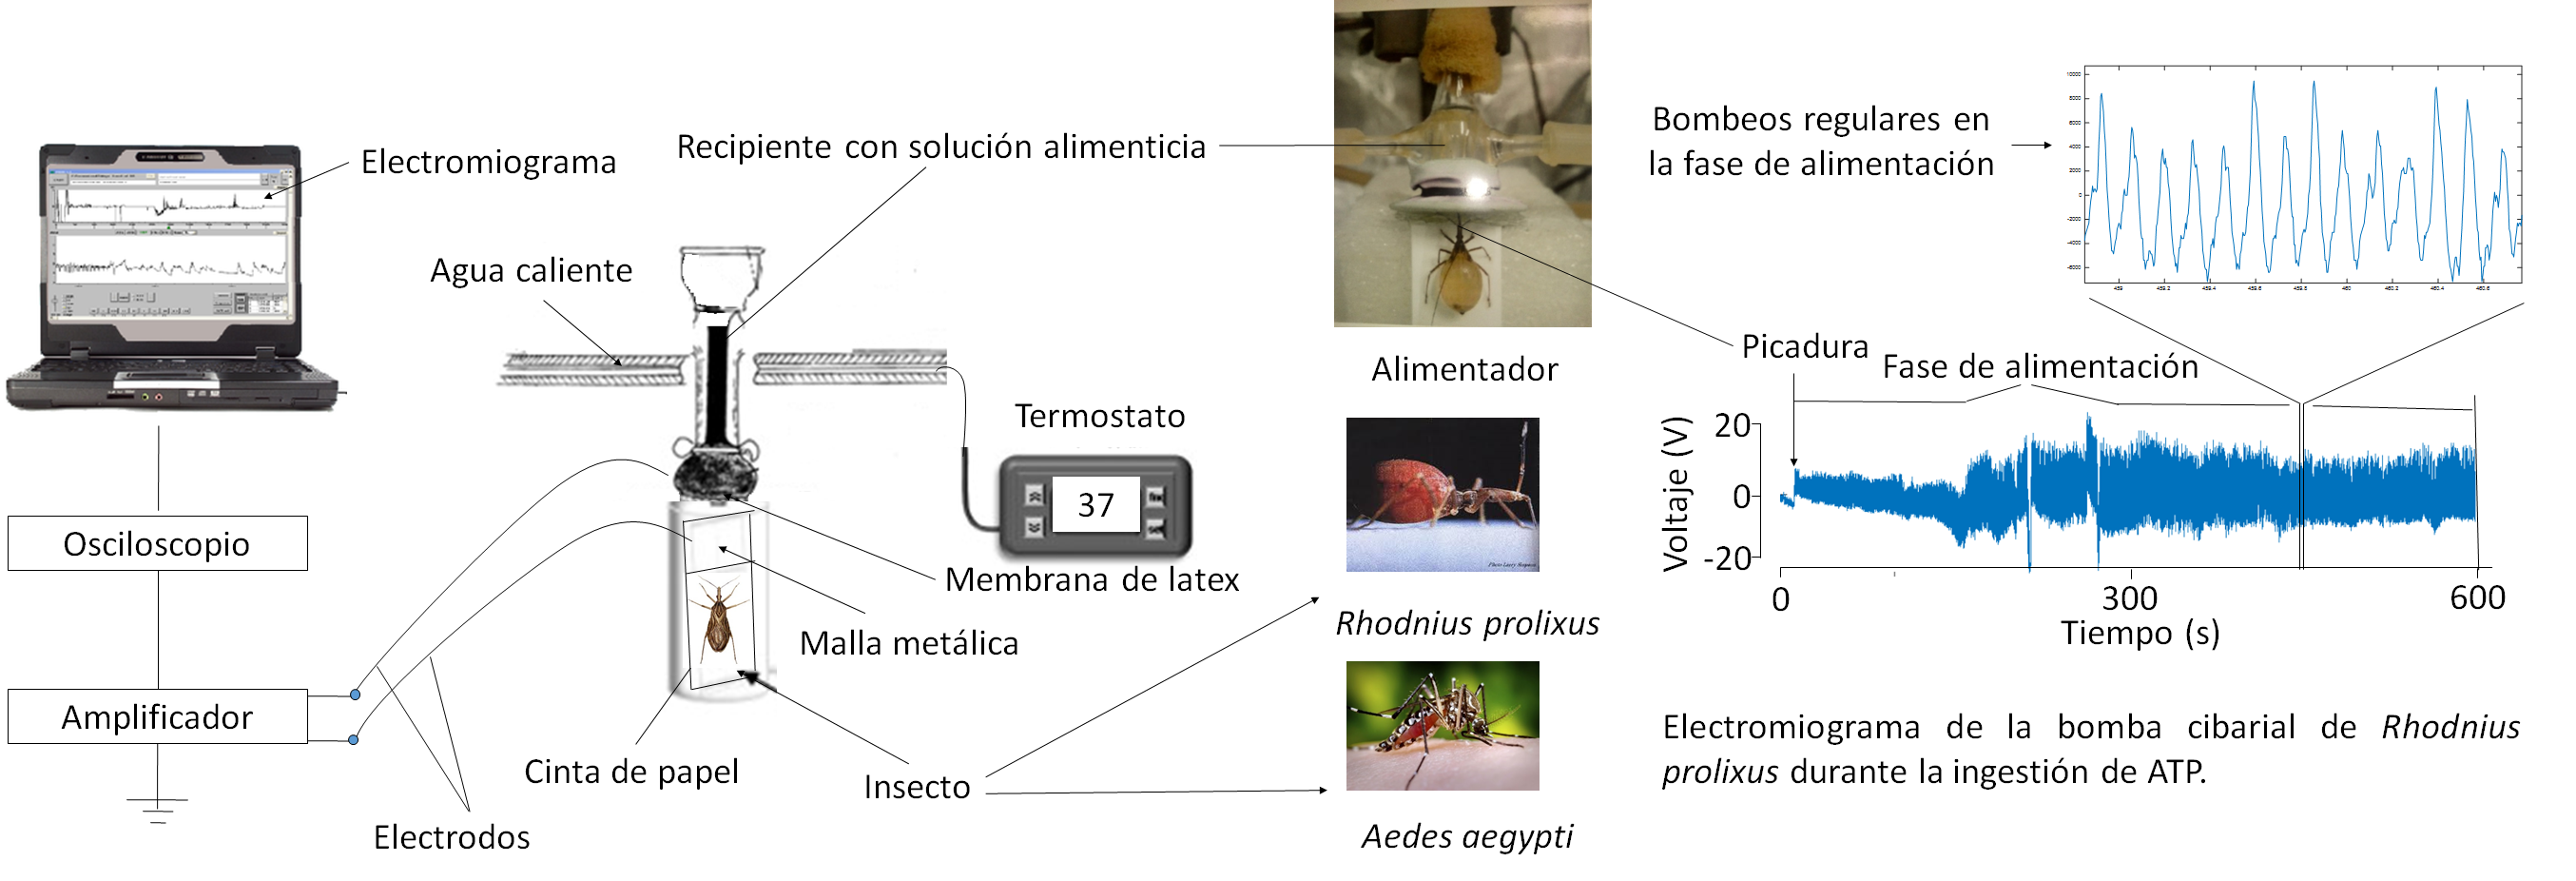
\includegraphics[trim={0cm 0cm 0cm 0cm}, clip,width=.5\textwidth]{./setup.png}
	\caption{Setup de la medición.}
	\label{setup}
\end{figure}


Se trabajaron con datos de laboratorio reales. Una serie temporal típica se puede ver en las figuras \ref{serieOrig} y \ref{serieOrig2}.

\begin{figure}[ht]
	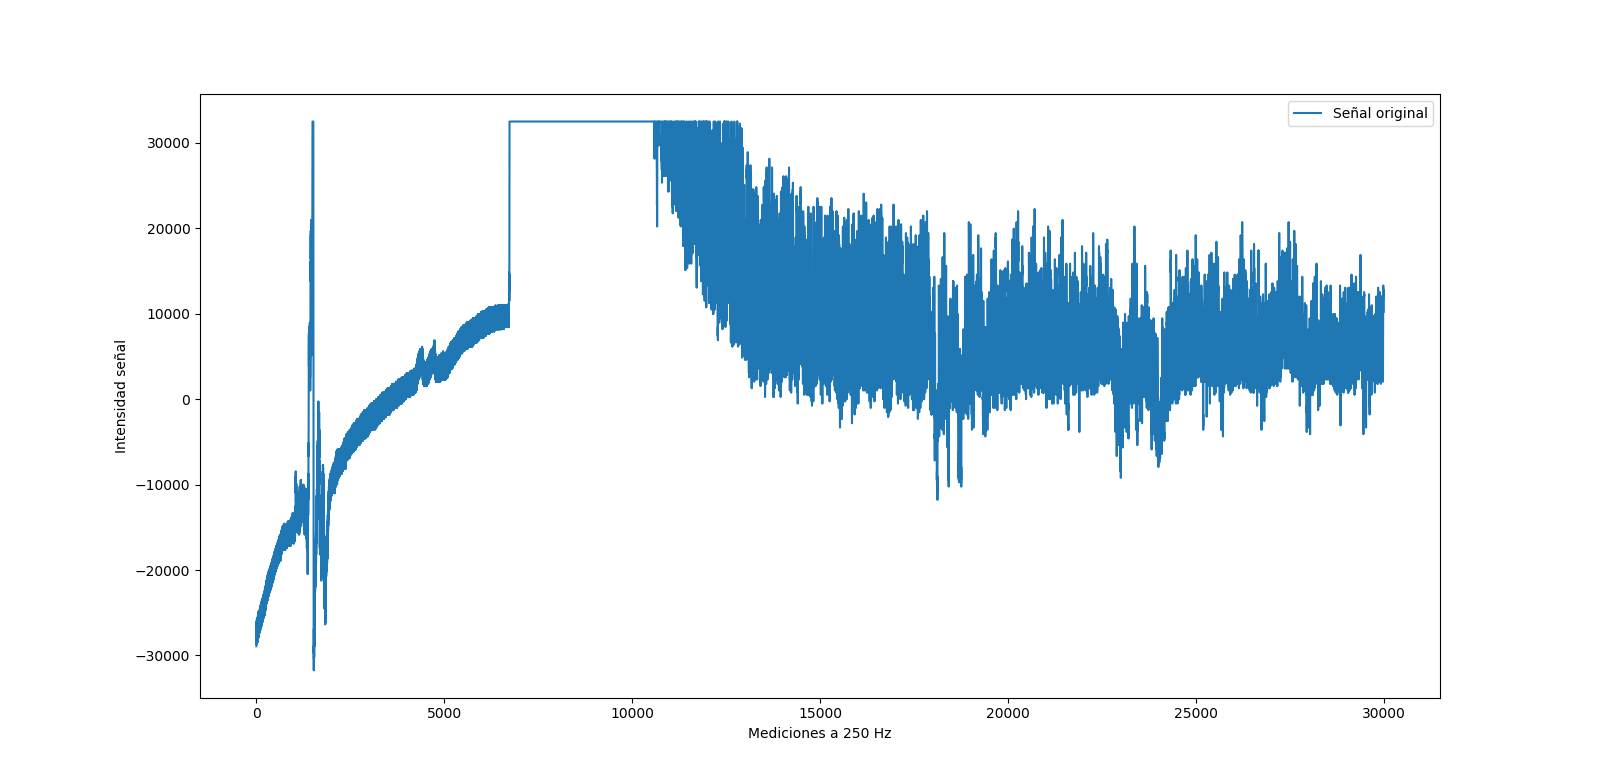
\includegraphics[trim={3cm 1cm 3cm 1cm}, clip,width=.5\textwidth]{./senialOrig.png}
	\caption{Serie de datos temporal típica.}
	\label{serieOrig}
\end{figure}
\begin{figure}[ht]
	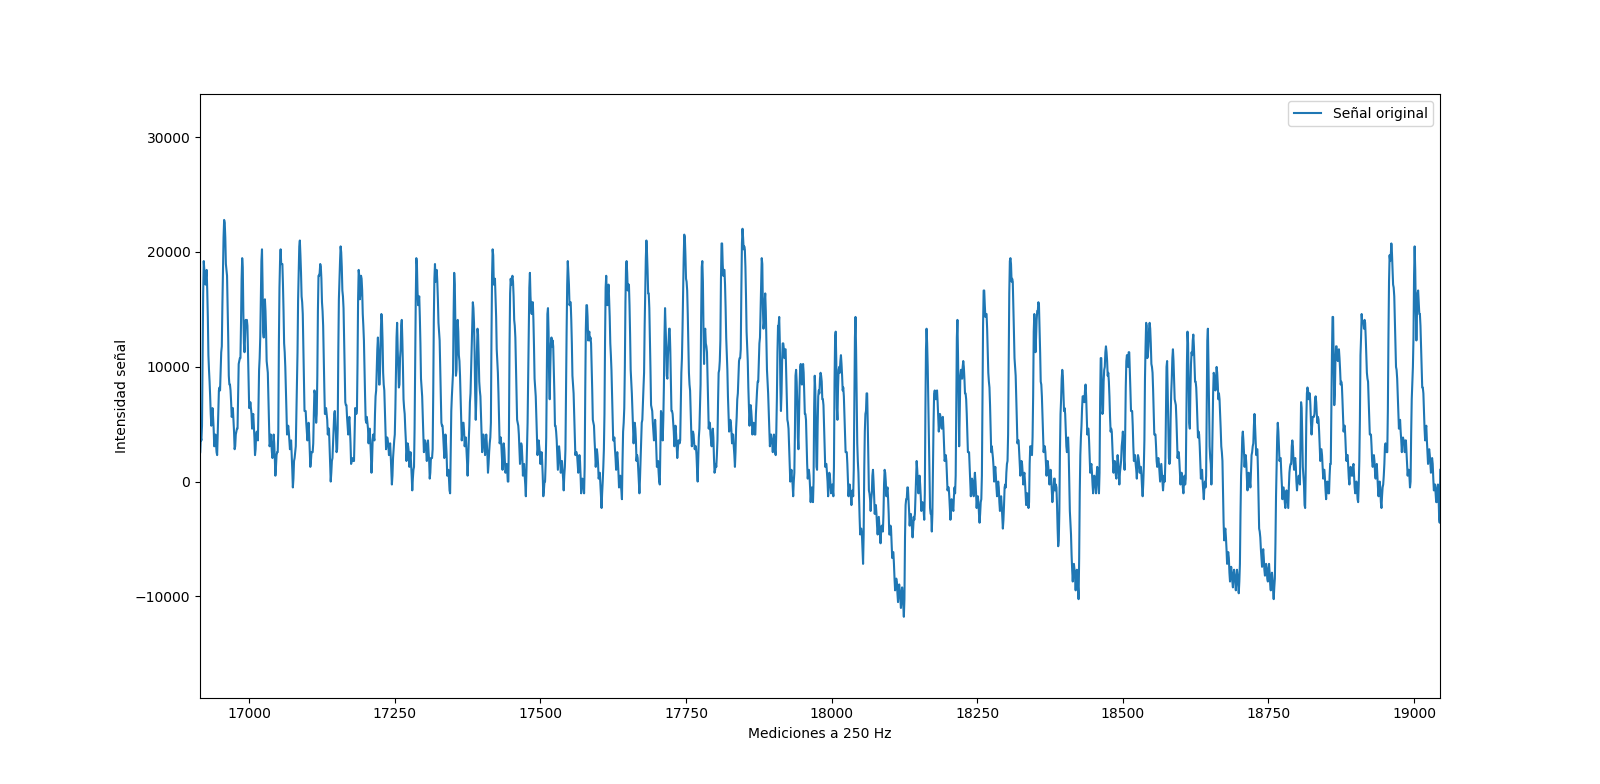
\includegraphics[trim={3cm 1cm 3cm 1cm}, clip,width=.5\textwidth]{./senial2Orig.png}
	\caption{Serie de datos temporal típica.}
	\label{serieOrig2}
\end{figure}

Como la serie temporal consta de la deriva típica proveniente de mediciones con aparatos electrónicos, como preprocesamiento a la señal para quitar esta deriva se utilizó el algoritmos BEADS (ver \cite{beads}). La serie luego de remover la deriva se puede ver en las figuras \ref{serieBeads} y \ref{serieBeads2}.

\begin{figure}[ht]
	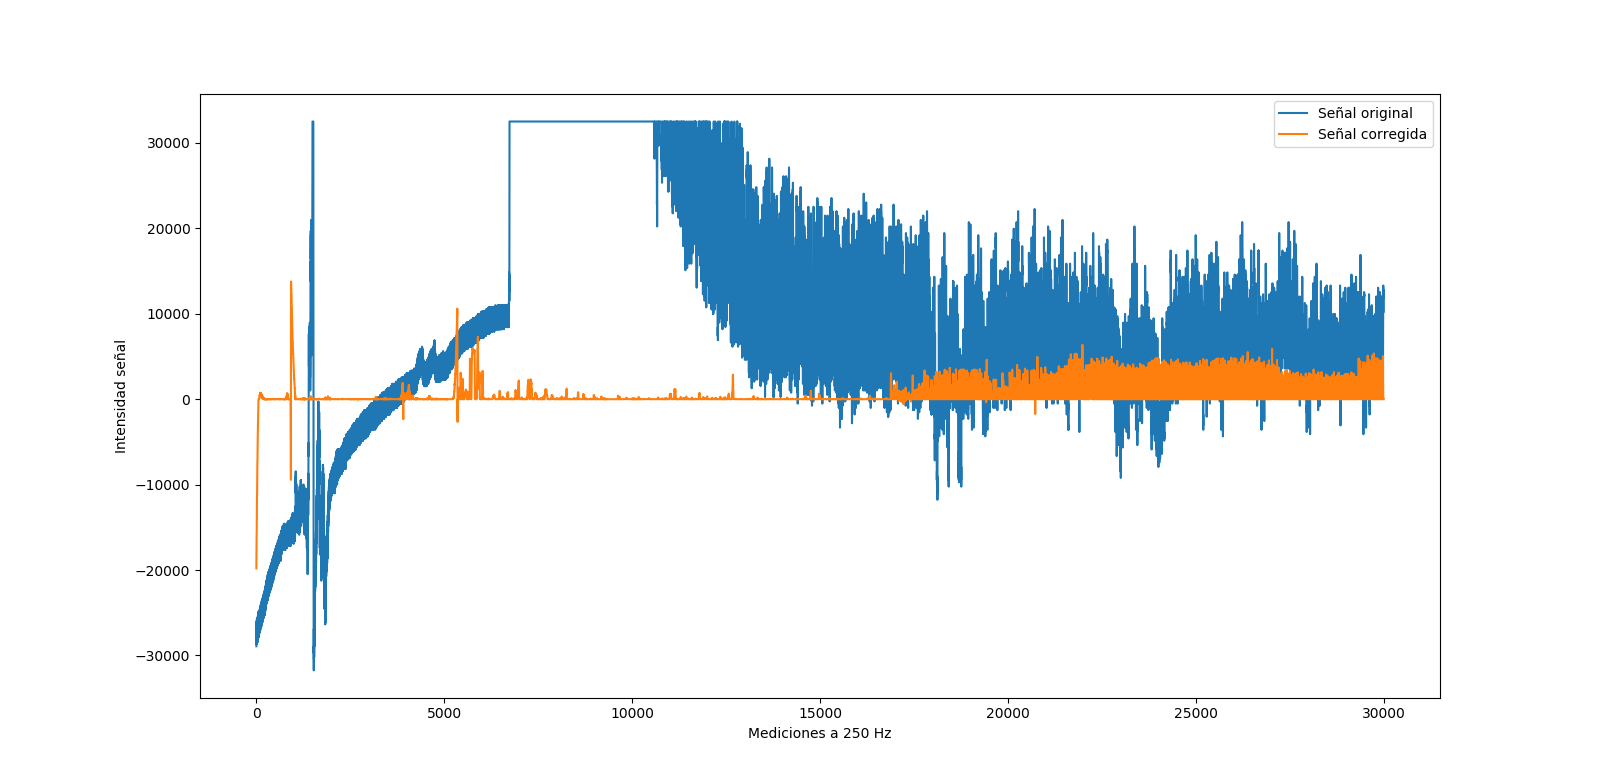
\includegraphics[trim={3cm 1cm 3cm 1cm}, clip,width=.5\textwidth]{./senial.png}
	\caption{Serie de datos temporal típica (azul) y corregida por BEADS (naranja).}
	\label{serieBeads}
\end{figure}
\begin{figure}[ht]
	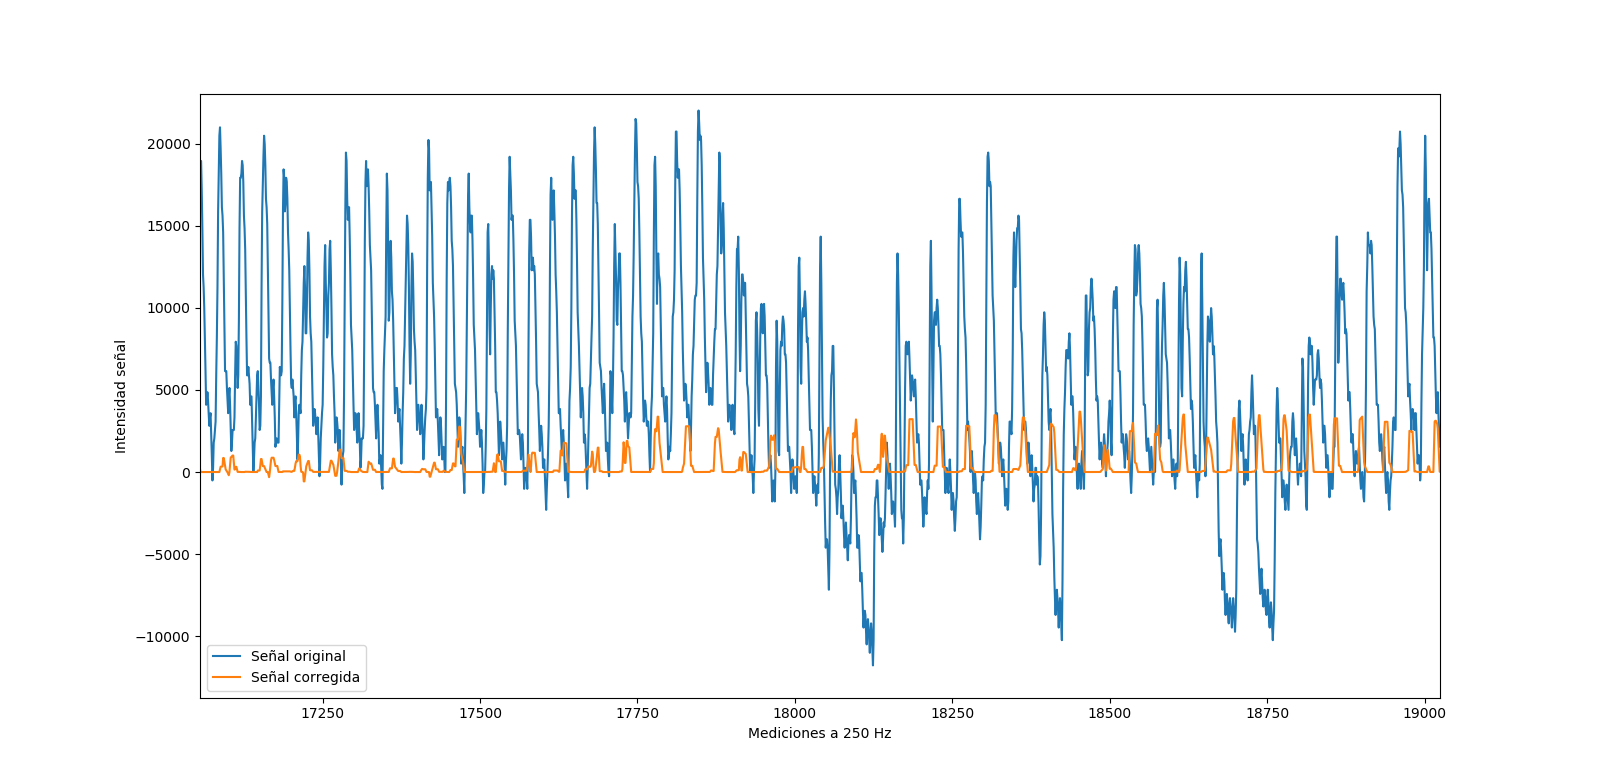
\includegraphics[trim={3cm 1cm 3cm 1cm}, clip,width=.5\textwidth]{./senial2.png}
	\caption{Serie de datos temporal típica (azul) y corregida por BEADS (naranja).}
	\label{serieBeads2}
\end{figure}

Posteriormente se dividió la serie temporal en pequeñas ventanas, cada una clasificada por Sí/No respecto al insecto comiendo. Se probaron con ventanas de 6, 1 y 0.5 segs. La figura \ref{serieVentanas} ilustra la situación.
\begin{figure}[h]
	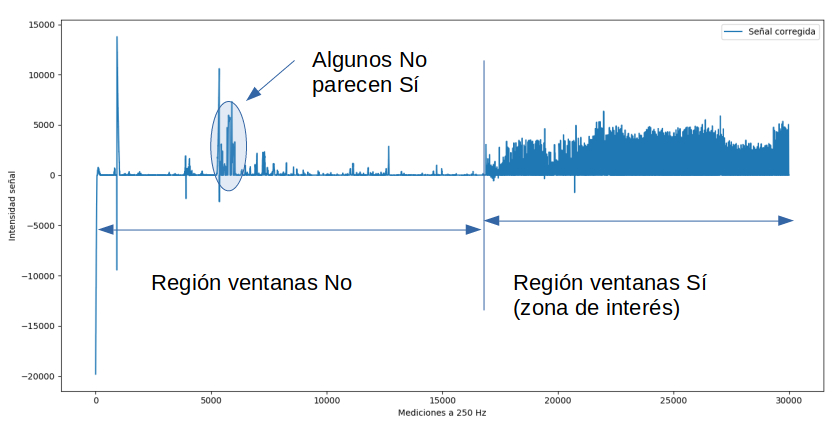
\includegraphics[trim={0cm 0cm 0cm 0cm}, clip,width=.5\textwidth]{./separacionVentanasBien.png}
	\caption{Regiones utilizadas para generar las ventanas de clasificación. Cada región consta de muchas ventanas.}
	\label{serieVentanas}
\end{figure}


\section{Redes y resultados}
Se probaron varias redes convolucionales, para los distintos anchos de ventanas. Por suerte se contaban con muchos datos (3000 para ventanas de 6 segundos y 18 mil para de 1 segundo).

Se particionaron los datos en 80/20\% train/test respectivamente, y se mezclaron aleatoriamente. Además siempre se trabajó con datasets previamente balanceados 50/50\% para cada clase respectivamente.

En general los resultados, medidos en accuracy, obtenidos fueron aceptables, de 90\% en adelante. El mejor resultado se obtuvo en ventanas de tamaño 1 seg. con una ConvNet de 3 convoluciones, 2 max poolings, y 3 FCs, el cual fue de un accuracy del 95-96\%. Además se normalizaron previamente los datos de entrada.

La figura \ref{clasif} ilustra el resultado respecto a épocas de entrenamiento.
\begin{figure}[h]
	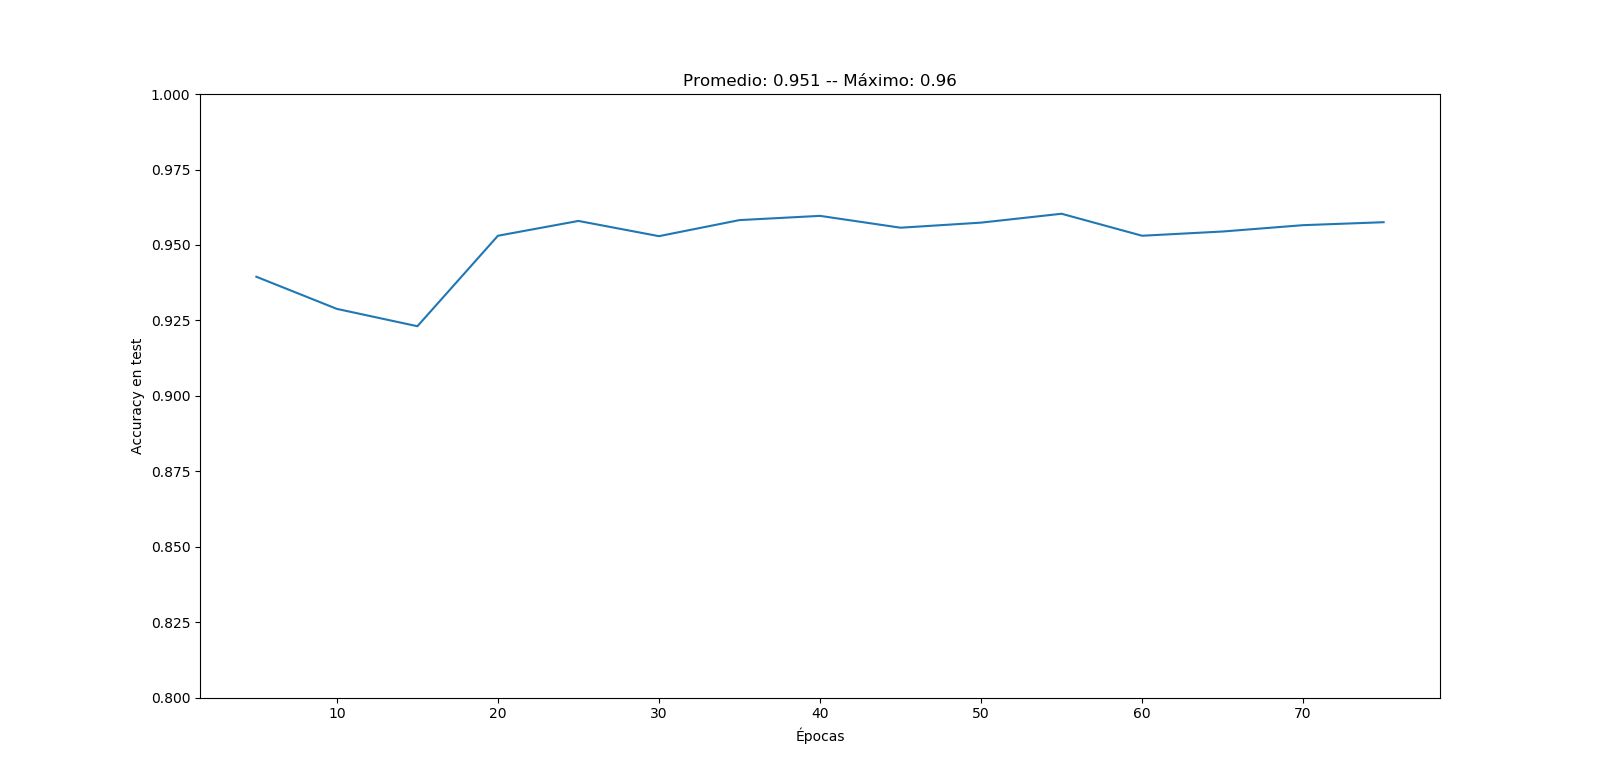
\includegraphics[trim={3cm 1cm 3cm 1cm}, clip,width=.5\textwidth]{./cnn_v7_1seg_normalizado_b5000.png}
	\caption{Mejor resultado de clasificación de ventanas, respecto al accuracy.}
	\label{clasif}
\end{figure}

%También se probó una red recurrente, obteniéndose un accuracy algo superior al 96\%.

Finalmente, y como prueba rápida de último momento, se probó clasificar utilizando las FFTs de las ventanas (parte real y compleja). El resultado también fue satisfactorio, como muestra la figura \ref{clasifFFT}, con un accuracy del 91-92\%.
\begin{figure}[h]
	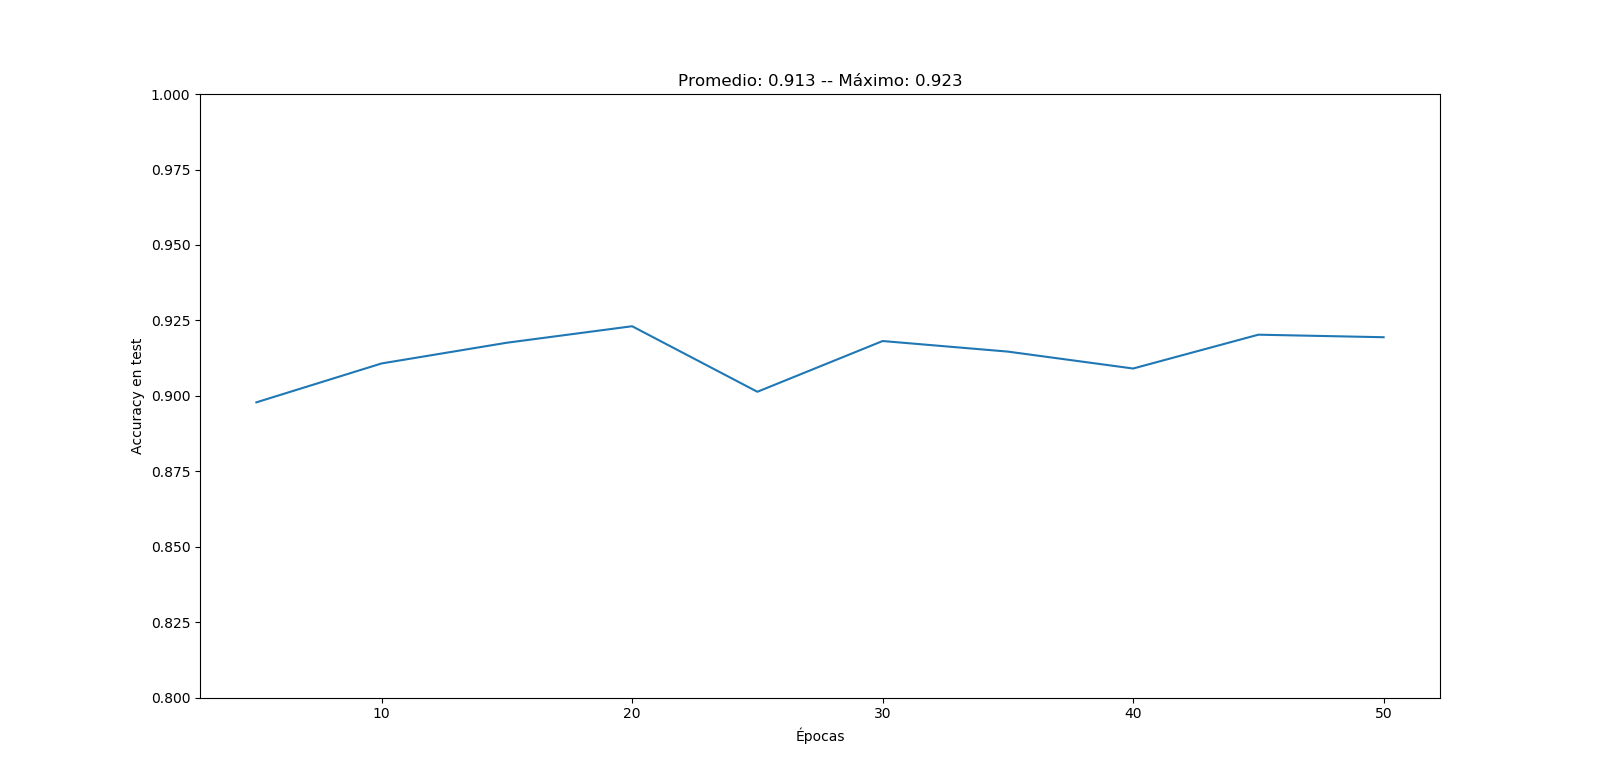
\includegraphics[trim={3cm 1cm 3cm 1cm}, clip,width=.5\textwidth]{./cnn_v7_1seg_normalizado_fft_b1000.png}
	\caption{Mejor resultado de clasificación de ventanas por FFTs, respecto al accuracy.}
	\label{clasifFFT}
\end{figure}


Posteriormente se probó otra red convolucional pero dilated, obteniéndose un accuracy algo mayor al 96\%. Esta red se entrenó por 30 épocas, y en la figura \ref{clasifDilated} se muestra el accuracy respecto a cada dato de test (800 en total).
\begin{figure}[h]
	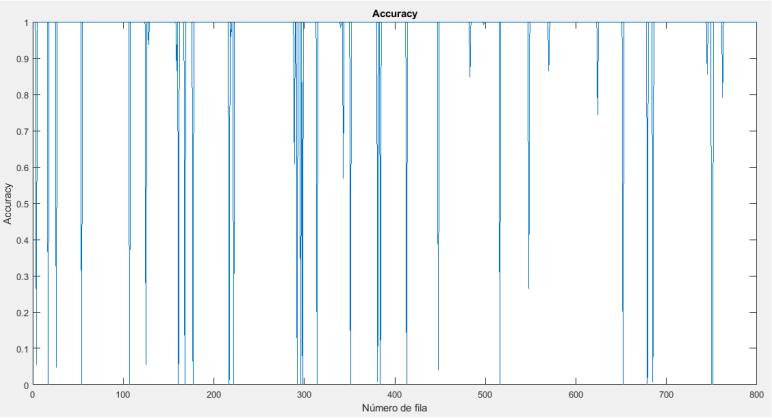
\includegraphics[trim={0cm 0cm 0cm 0cm}, clip,width=.5\textwidth]{./convDilated.png}
	\caption{Resultado clasificación por accuracy con la convolucional dilated.}
	\label{clasifDilated}
\end{figure}

Y finalmente se probó una red recurrente, obteniéndose un accuracy del 93\% como muestra la figura \ref{clasifRecurrent}.
\begin{figure}[h]
	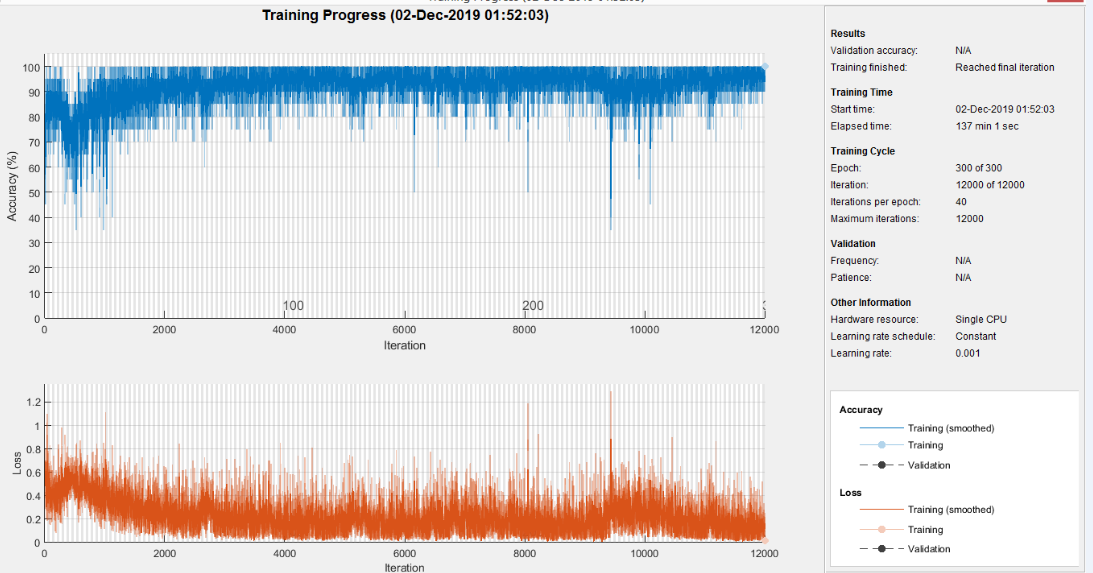
\includegraphics[trim={0cm 0cm 0cm 0cm}, clip,width=.5\textwidth]{./recurrent.png}
	\caption{Resultado clasificación por accuracy con la recurrente.}
	\label{clasifRecurrent}
\end{figure}


\section{Cómo seguir}
Quedaron varias cuestiones a probar o mejorar, a saber:
\begin{itemize}
		\item Probar con otras arquitecturas/parámetros para las CNNs. En particular achicar el tamaño de los filtros en las convolucionales.
\item Probar otras Recurrentes.
\item Input con series temporal + FFTs.
\item Ensambles.
\item Barrer el tamaño de la ventana más exhaustivamente.
\item Barrer el tamaño de mini-batch más exhaustivamente.
\item Reconocer más patrones en los registros, por ejemplo:
\begin{itemize}
%	\item Número de veces que pica el insecto.
	\item Cantidad y tiempo de cada evento de picado/no-picado.
%	\item Número de bombeos totales.
	\item Tiempo, frecuencia, amplitud media y cantidad de bombeos. 
\end{itemize}
\item Utilizar la matriz de confusión como métrica de performance, para detectar mejor dónde está fallando la clasificación.

\end{itemize}


\section{Arquitecturas}
\subsection{ConvNets}
Las convolucionales se utilizaron variantes de:
	\begin{itemize}
	\item Input: ventanas de cant. seg. corresp. (por 250 Hz de sampleo).
	\item Convolucional 1D de 5x60 (stride=1, padding=30) + ReLu
%	\item ReLu
	\item Convolucional 1D de 10x30 (stride=2, padding=30)
	\item Max Pooling de 2 + ReLu
%	\item ReLu 
	\item Convolucional 1D de 20x15 (stride=2, padding=30)
	\item Max Pooling de 2 + ReLu
%	\item ReLu
	\item FC de 580 a 300 + tanh
	\item FC de 300 a 100 + tanh
	\item FC de 100 a Sí/No
\end{itemize}
Las variantes esencialmente incluyeron pruebas sin la última convolucional, y también sin al FC intermedia.

\subsection{ConvNet Dilated}
Para la convolucional dilated la arquitectura fue:

%\begin{figure}[h]
	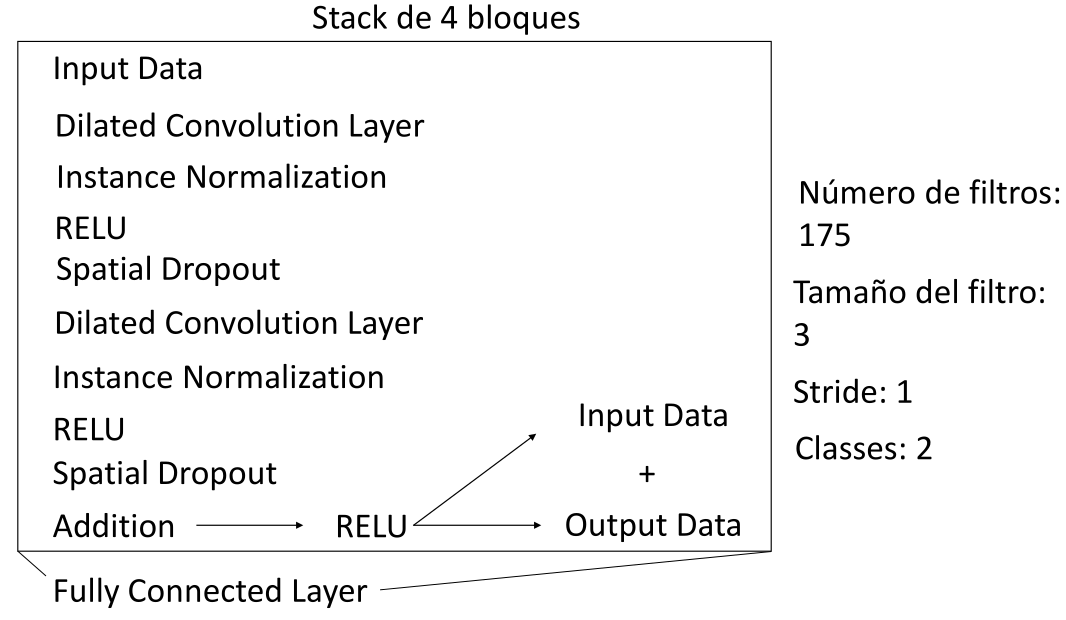
\includegraphics[trim={0cm 0cm 0cm 0cm}, clip,width=.5\textwidth]{./arqDilated.png}
%	\caption{Resultado clasificación por accuracy con la recurrente.}
%	\label{clasifRecurrent}
%\end{figure}

\subsection{Recurrente}
Y para la recurrente la arquitectura fue:

%\begin{figure}[h]
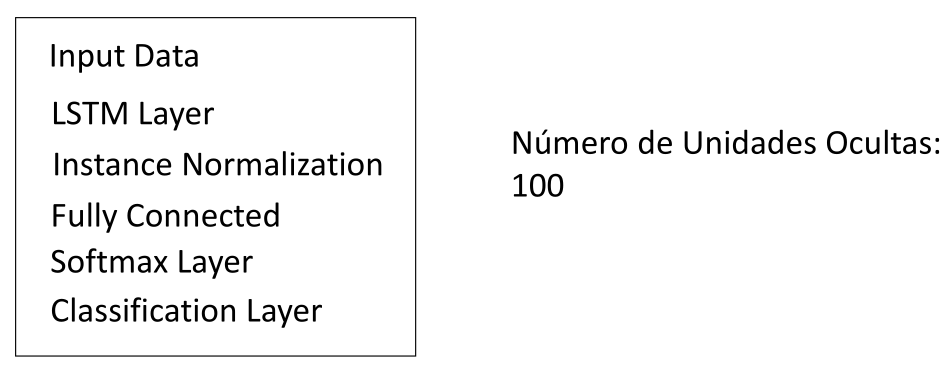
\includegraphics[trim={0cm 0cm 0cm 0cm}, clip,width=.5\textwidth]{./arqRecurrent.png}



\begin{thebibliography}{9}

\bibitem{beads}
Xiaoran Ning; Ivan W.Selesnick; Laurent Duval; \emph{Chromatogram baseline estimation and denoising using sparsity (BEADS)};\\
\small\url{https://doi.org/10.1016/j.chemolab.2014.09.014}
%\small\url{http://www.laurent-duval.eu/siva-beads-baseline-background-removal-filtering-sparsity.html}
%Cengage Learning, 7 ed., 2012.\\
%Secciones 17.1 y 17.2


\end{thebibliography}




\end{document}